\section{Langevin Dynamics Inspired Samplers and Integrators}

    In addition to Hamiltonian dynamics, we can model the dynamics of molecular systems with Langevin dynamics. This model relies on the fact that a real world molecular system is unlikely to be present in a vacuum (there may be friction, jostling, etc.). There are two types of Langevin dynamics: overdamped and underdamped. The \textbf{Gibbs measure} mentioned below is an invariant distribution of this random process, similar to a stationary distribution of a Markov chain. That is, if we ran the model for an infinite amount of time, the Gibbs measure would be the density representing the probability of finding that particle at a certain location at any point in time. 
    \begin{enumerate}
      \item The overdamped Langevin equation does not rely on the momenta. 
      \begin{equation}
        \mathbf{\dot{q}} = - \nabla U(\mathbf{q}) + \sqrt{2 \beta^{-1}} \dot{W}
      \end{equation}
      Its Gibbs measure (invariant distribution) is 
      \begin{equation}
        \pi(\boldsymbol{\theta}) = \frac{1}{Z} \exp\big( - \beta U(\mathbf{q})\big), \text{ where } Z = \int \exp\big( - \beta U(\mathbf{q})\big)\; dq
      \end{equation}
      More precisely, given that the path $\mathbf{q}(t)$ at time $t$ is distributed according to (parameterized) density $\rho_t$, $\rho_t \rightarrow \frac{1}{Z} e^{-\beta U(\mathbf{q})}$ as $t \rightarrow +\infty$. 
      \item The underdamped Langevin equation can be interpreted as a Hamiltonian model, with the additional $- \gamma \mathbf{p} + \sqrt{2\gamma \beta^{-1}} \dot{W}$ term representing the interaction of the Hamiltonian system with an outside environment (called a heat bath or thermostat). 
      \begin{align*}
        \mathbf{\dot{q}} & = \mathbf{M}^{-1} \mathbf{p} \\
        \mathbf{\dot{p}} & = - \nabla U(\mathbf{q}) - \gamma \mathbf{p} + \sqrt{2\gamma \beta^{-1}} \mathbf{M}^{1/2} \dot{W}
      \end{align*}
      The $\gamma$ is the damping constant and $\beta$ is the inverse temperature. We can think of the term $-\gamma \mathbf{p}$ as the damping/dissipative term which "drags" the momentum $\mathbf{p}$ to $0$. The higher the $\gamma$, the stronger this drag. As $\gamma$ grows, the system spans from the inertial all the way to the diffusive (aka Brownian) regime. The term $\sqrt{2 \gamma \beta^{-1}} \dot{W}$ is the random term, which increases as temperature increases. It has invariant distribution 
      \begin{equation}
        \pi(\boldsymbol{q}, \boldsymbol{p}) = \frac{1}{Z} \exp\big( -\beta \big[ U(\mathbf{q}) + \frac{1}{2} |\mathbf{p}|^2\big] \big)
      \end{equation}
    \end{enumerate}
    To understand the relationship between the overdamped and underdamped Langevin equations and the physical systems that they represent, we can think of the overdamped equation as a limit of the underdamped one. As we set $\gamma \rightarrow +\infty$ (followed by an appropriate time scale), the underdamped Langevin equation would converge to the overdamped because the friction term would become very large, causing the momenta to dissipate instantaneously. Another way to describe this limit is to incorporate a mass matrix $\mathbf{M}$ into the underdamped: 
    \begin{align*}
      \mathbf{\dot{q}} & = \mathbf{M}^{-1} \mathbf{p} \\
      \mathbf{\dot{p}} & = - \nabla U(\mathbf{q}) - \gamma \mathbf{M}^{-1} \mathbf{p} + \sqrt{2\gamma \beta^{-1}} \dot{W}
    \end{align*}
    If we let $\mathbf{M} \rightarrow \mathbf{0}$, then we can see that the dissipative term $- \gamma \mathbf{M}^{-1}  \mathbf{p}$ will grow very large, which leads to convergence to the overdamped equation. 

    The overdamped Langevin equation is usually used to represent Brownian motion, similar to a random walk, in which there is no memory of the momenta from one time to another. The underdamped Langevin equation incorporates the momenta $\mathbf{p}$, and so the trajectory would be a lot smoother. 

    The underdamped equation has a lot nicer properties that allows us to sample efficiently. For example, when we have a double well potential $U(q)$ with the associated Gibbs measure, sampling from this potential with an overdamped integrator can cause problems. The overdamped integrator does not remember momentum, and so when crossing the energy barrier it tends to go over and recross back due to the random term. 
    \begin{center}
      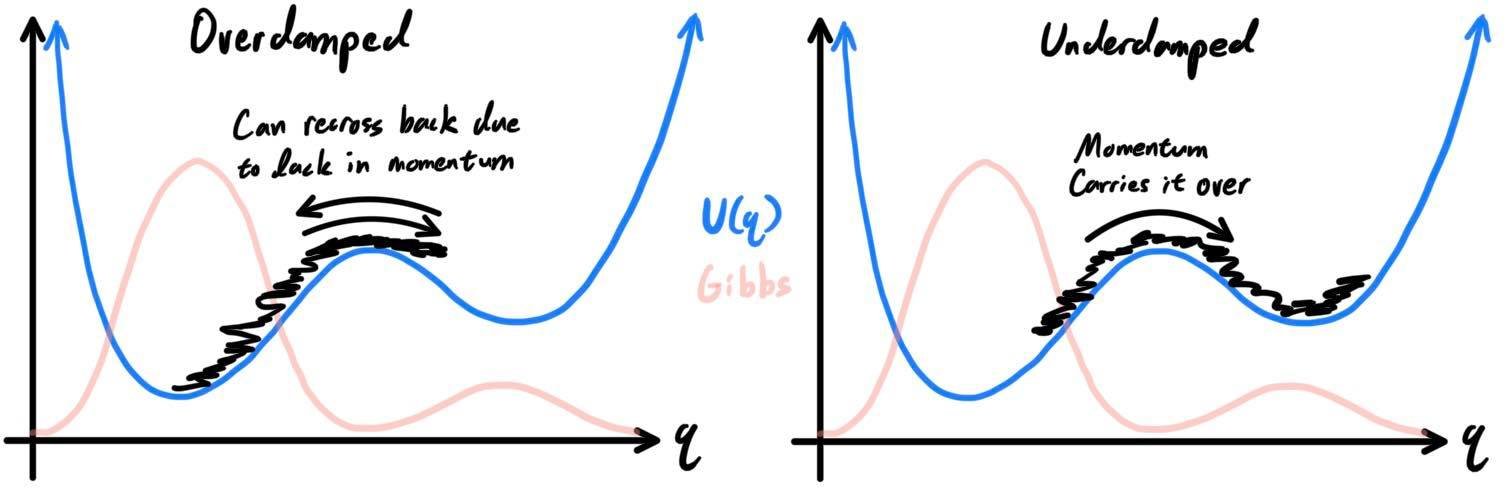
\includegraphics[scale=0.25]{img/double_well.jpg}
    \end{center}
    For the underdamped, the momentum is remembered and so when we reach over the barrier, the momentum that accelerates the particle across the well, along with the momentum that accelerates it down the well as soon as it is across, carries the particle into the other well. The choice of our friction coefficient $\gamma$ will determine how often we transition one stable state (well) to the other stable state. Choosing the right $\gamma$ is very important when sampling. 
    \begin{enumerate}
      \item If $\gamma$ is too large, we will have very similar dynamics to the overdamped Langevin equation (lots of randomness and potential recrossings), which is not ideal.
      \item If $\gamma$ is too small, it will be very similar to Hamiltonian dynamics, with a very small dissipative and random forces. It will end up just crossing back and forth smoothly and deterministically. 
    \end{enumerate}


    To compare Hamiltonian, underdamped, and overdamped dynamics, let us take a look at the phase space of the double well, with equi-Hamiltonian level sets. 
    \begin{enumerate}
      \item A Hamiltonian flow will precisely be along the level sets, since the Hamiltonian is conserved. 
      \item An underdamped Langevin flow (with $\gamma$ not too large) will move slowly between level sets. It is important not to set $\gamma$ to small since then our flow would transition very slowly between level sets and not explore our phase space very quickly. 
      \item An overdamped Langevin flow (or underdamped with large $\gamma$) will move very quickly between level sets, leading to a random walk behavior. 
    \end{enumerate}
    \begin{center}
      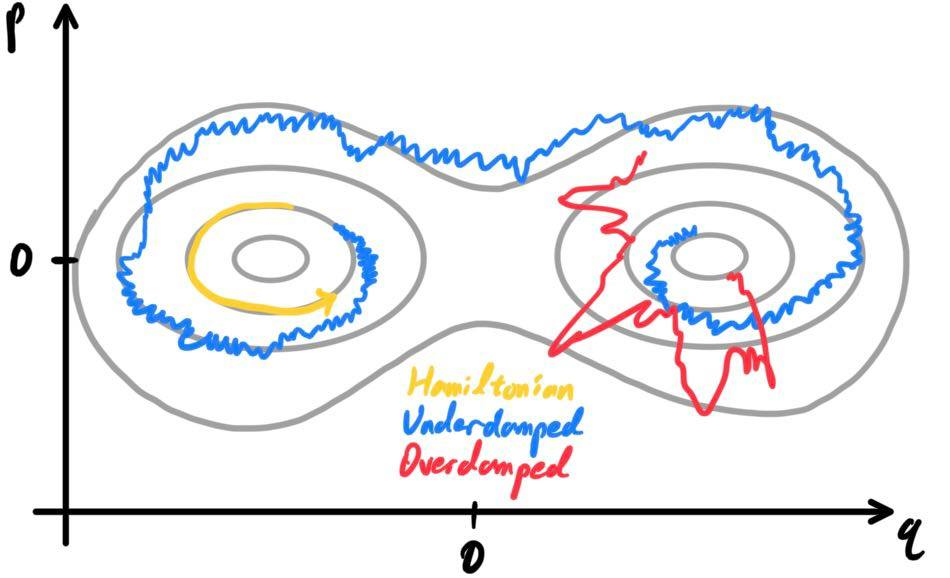
\includegraphics[scale=0.25]{img/phase_space.jpg}
    \end{center}

  \subsection{SGLD}

    Now if we add Gaussian noise to SGD, then we get \textit{Stochastic Gradient Langevin Dynamics (SGLD)} sampler, which is the discretized form of the overdamped Langevin equation 
    \begin{equation}
      \mathbf{\dot{q}} = - M^{-1} \nabla_\mathbf{q} U(\mathbf{q}) + \sqrt{2 \beta^{-1}} M^{-1/2} \dot{W}
    \end{equation}
    where $M$ is the mass matrix, $\beta$ the inverse temperature, and $\dot{W}$ a Weiner process. If the gradient computations are exact, then SGLD reduces to the \textit{Langevin Monte Carlo} algorithm. This algorithm is also a reduction of Hamiltonian Monte Carlo, consisting of a single leapfrog step proposal rather than a series of steps. Since SGLD can be formulated as a modification of both SGD and MCMC methods, it lies at the intersection between optimization and sampling algorithms. The method maintains SGD's ability to quickly converge to regions of low cost while providing samples to facilitate posterior inference. 

    If we set the mass matrix to be $I$, we can update $\mathbf{q}$ according to the following discretization. 
    \begin{equation}
      \mathbf{q}_{t+1} = \mathbf{q}_t - \nabla_{\mathbf{q}} U(\mathbf{q}_t) + \sqrt{2 \beta^{-1}} \, \boldsymbol{\epsilon}, \;\;\;\;\; \boldsymbol{\epsilon} \sim \mathcal{N}(\mathbf{0}, \mathbf{I})
    \end{equation}

    \begin{algorithm}
      \caption{SGLD}\label{alg:sgld}
      \begin{algorithmic}

      \Require Initial $\boldsymbol{\theta}_0$, Stepsize function $h(t)$, Minibatch size $m$

      \For{$t = 0$ to $T$}
          \State $\hat{g}(\theta_t) \gets \nabla_\theta \log{p(\theta_t \mid M_m(\mathcal{D}))}$
          \State $\epsilon_t \sim \mathcal{N}(0, I)$
          \State $\theta_{t+1} \gets \theta_t + h(t) \cdot \hat{g}(\theta_t) + \sqrt{2 h(t) \beta^{-1}} \, \epsilon_t$
      \EndFor

      \end{algorithmic}
    \end{algorithm}

    We can incorporate the mass matrix, which is approximated by the precision of the log posterior ($M^{-1} = \Sigma$), for adapting (along with preconditioning if needed). This would result in the discretized step: 
    \begin{equation}
      \mathbf{q}_{t+1} = \mathbf{q}_t - M^{-1} \nabla_{\mathbf{q}} U(\mathbf{q}_t) + \sqrt{2 \beta^{-1}} M^{-1} \, \boldsymbol{\epsilon}
    \end{equation}

    \begin{algorithm}
      \caption{Adaptive SGLD}\label{alg:adaptive_sgld}
      \begin{algorithmic}

      \Require Initial $\boldsymbol{\theta}_0$, Stepsize function $h(t)$, Minibatch size $m$, Adaptation burn-in $B$, Adaptation frequency $U$
      \State $\mu_0^{\mathrm{emp}} \gets 0$
      \State $\Sigma_0 \gets I$
      \State $\Sigma_0^{\mathrm{emp}} \gets I$

      \For{$t = 0$ to $T$}
          \State $\hat{g}(\theta_t) \gets \nabla_\theta \log{p(\theta_t \mid M_m(\mathcal{D}))}$
          \State $\epsilon_t \sim \mathcal{N}(0, \Sigma^t)$
          \State $\theta_{t+1} \gets \theta_t + h(t) \, \Sigma_t \, \hat{g}(\theta_t) + \sqrt{2 h(t) \beta^{-1}} \, \epsilon_t$
          
          \State $\Sigma^\mathrm{emp}_{t+1} \gets \frac{1}{t+1} \big[(\theta^{t+1} - \mu_t) (\theta^{t+1} - \mu_t)^T - \Sigma^\mathrm{emp}_t \big]$
          \State $\mu_{t+1}^\mathrm{emp} \gets \mu_t + \frac{1}{t+1} [ \theta_{t+1} - \mu_t ]$
          
          \If{$t > B$ and $t$ is divisible by $U$}
              \State $\Sigma_{t+1} \gets \Sigma_{t+1}^{\mathrm{emp}}$
          \EndIf
      \EndFor

      \end{algorithmic}
    \end{algorithm}

  \subsection{MALA}

    We can slightly modify SGLD to get the \textit{Metropolis Adjusted Langevin Algorithm (MALA)} sampler, which has two differences from SGLD: 
    \begin{enumerate}
      \item SGLD uses a minibatch approximation of the gradient (hence the name stochastic), while MALA always uses the entire dataset.
      \item MALA has an additional Metropolis accept/reject step on the proposal state, while SGLD always "accepts" the new state.
    \end{enumerate}
    For the sake of conciseness, we will provide the adaptive MALA algorithm. 

    \begin{algorithm}
      \caption{Adaptive MALA}\label{alg:adaptive_mala}
      \begin{algorithmic}

      \Require Initial $\boldsymbol{\theta}_0$, Stepsize function $h(t)$, Minibatch size $m$, Adaptation burn-in $B$, Adaptation frequency $U$
      \State $\mu_0^{\mathrm{emp}} \gets 0$
      \State $\Sigma_0 \gets I$
      \State $\Sigma_0^{\mathrm{emp}} \gets I$

      \For{$t = 0$ to $T$}
          \State $\hat{g}(\theta_t) \gets \nabla_\theta \log{p(\theta_t \mid \mathcal{D})}$
          \State $\epsilon_t \sim \mathcal{N}(0, \Sigma^t)$
          \State $P_{t+1} \gets \theta_t + h(t) \, \Sigma_t \, \hat{g}(\theta_t) + \sqrt{2 h(t) \beta^{-1}} \, \epsilon_t$ 
          
          \If{$\log{p(P_{t+1} \mid \mathcal{D})} \geq \log{p(\theta_t \mid \mathcal{D})}$} 
              \State $\theta_{t+1} \gets P_{t+1}$
          \Else 
              \State $\delta \sim \mathrm{Uniform}[0, 1]$ 
              \If{$\delta < \log{p(P_{t+1} \mid \mathcal{D})} / \log{p(\theta_t \mid \mathcal{D})}$}
                  \State $\theta_{t+1} \gets P_{t+1}$ 
              \Else 
                  \State $\theta_{t+1} \gets \theta_t$
              \EndIf
          \EndIf
          
          \State $\Sigma^\mathrm{emp}_{t+1} \gets \frac{1}{t+1} \big[(\theta^{t+1} - \mu_t) (\theta^{t+1} - \mu_t)^T - \Sigma^\mathrm{emp}_t \big]$
          \State $\mu_{t+1}^\mathrm{emp} \gets \mu_t + \frac{1}{t+1} [ \theta_{t+1} - \mu_t ]$
          
          \If{$t > B$ and $t$ is divisible by $U$}
              \State $\Sigma_{t+1} \gets \Sigma_{t+1}^{\mathrm{emp}}$
          \EndIf
      \EndFor

      \end{algorithmic}
    \end{algorithm}

  \subsection{Langevin Numerical Integrators}

    \subsubsection{Euler-Mayurama Method}

      The Euler-Mayurama integrator models Brownian dynamics/overdamped Langevin dynamics. We update the position vector $\mathbf{q}$ with a single timestep: 
      \begin{equation}
        \mathbf{q}_{k+1} = \mathbf{q}_k + h \mathbf{M}^{-1} \nabla U(\mathbf{q}_k) + \sqrt{2 h k_B T} \mathbf{M}^{-1/2} \mathbf{R}_k
      \end{equation}
      where $\mathbf{R}_k$ are vectors of standard independent Gaussian $\mathcal{N}(0, I)$ variables, resampled at each step. Since $k_B$ is the Boltzmann constant, we can set $\beta = (k_B T)^{-1}$ to be the \textbf{inverse temperature} parameter, reducing the above to 
      \begin{equation}
        \mathbf{q}_{k+1} = \mathbf{q}_k + h \mathbf{M}^{-1} \nabla U(\mathbf{q}_k) + \sqrt{2 h \beta^{-1}} \mathbf{M}^{-1/2} \mathbf{R}_k
      \end{equation}
      This EM discretized scheme has an invariant measure $\hat{\pi}_h$ that is also an approximation of the true Gibbs measure $\pi$ of the original Langevin equation. We subscript it with the step size $h$ since convergence will be dependent on $h$. 
      \begin{equation}
        \hat{\pi}_h (\mathbf{q}) = \pi(\mathbf{q}) + \mathcal{O}(h)
      \end{equation}
      We can interpret the $\mathcal{O}(h)$ term as a term $\rho(\mathbf{q}) h$ (where $\rho$ is some density) that vanishes linearly as $h \rightarrow 0$. 

    \subsubsection{Leimkuhler-Matthews Method}

      The Leimkuhler-Matthews method also finds discretized solutions to Brownian dynamics, with position update of 
      \begin{equation}
        \mathbf{q}_{k+1} = \mathbf{q}_k + h \mathbf{M}^{-1} \nabla U(\mathbf{q}_k) + \sqrt{2 h \beta^{-1}} \mathbf{M}^{-1/2} \bigg( \frac{\mathbf{R}_k + \mathbf{R}_{k-1}}{2} \bigg)
      \end{equation}

    \subsubsection{BAOAB Method}

      The BAOAB method is a symplectic integrator that models an undampened Langevin flow, with the following steps per timestep: 
      \begin{align*}
        \mathbf{p}_{k + 1/2} & = \mathbf{p}_k - \frac{h}{2} \nabla U(\mathbf{q}_k) \\
        \mathbf{q}_{k + 1/2} & = \mathbf{q}_k + \frac{h}{2} \mathbf{M}^{-1} \mathbf{p}_{k + 1/2} \\
        \mathbf{\hat{p}}_{k + 1/2} & = e^{-h \gamma} \mathbf{p}_{k + 1/2} + \sqrt{\beta^{-1} (1 - e^{-2\gamma h})} \mathbf{M}^{1/2} \mathbf{R}_k \\ 
        \mathbf{q}_{k + 1} & = \mathbf{q}_{k + 1/2} + \frac{h}{2} \mathbf{M}^{-1} \mathbf{\hat{p}}_{k + 1/2} \\
        \mathbf{p}_{k + 1} & = \mathbf{\hat{p}}_{k + 1/2} - \frac{h}{2} \nabla U(\mathbf{q}_{k + 1}) 
      \end{align*}
      where $\mathbf{R}_k$ are vectors of standard independent Gaussian $\mathcal{N}(0, I)$ variables, resampled at each step. Notice that the O step incorporates the randomness within this integrator. 
      BAOAB is a discretization of an underdamped Langevin flow, but BAOAB with an extremely large $\gamma$ would be similar to a discretization of an overdamped Langevin flow. There are other BAO splitting schemes, such as OBABO, OABAO, and ABOBA, but BAOAB is the best. 

      Recall that the true invariant measure of underdamped Langevin equations is $\pi(\mathbf{q}, \mathbf{p}) = \frac{1}{Z} \exp \big( -U(\mathbf{q}) + \frac{1}{2} |\mathbf{p}|^2 \big)$. BAOAB is a second-order scheme, meaning that the invariant measure $\hat{\pi}_h$ of this discretized scheme is a second order approximation of $\pi$. With some analysis, we can see that $\hat{\pi}$ is of order 2 (in fact, the BAO methods are all of order 2). 
      \begin{align*}
        \hat{\pi}_h (\mathbf{q}, \mathbf{p}) & = \pi(\mathbf{q}, \mathbf{p}) + C h^2 f_2 (\mathbf{q}, \mathbf{p}) \pi(\mathbf{q}, \mathbf{p}) + \mathcal{O}(h^4) \\
        & = \pi(\mathbf{q}, \mathbf{p}) + \mathcal{O}(h^2)
      \end{align*}
      where $f_2$ is some function such that $\mathbb{E}_\mathbf{p} [f_2] = 0$. But we are typically interested in just $\mathbf{q}$ when looking at the Gibbs density of a system, so we look at the marginal measure of $\mathbf{q}$: $\hat{\pi}_h (\mathbf{q}) = \int_\mathbf{p} \hat{\pi}_h (\mathbf{q}, \mathbf{p})\, d\mathbf{p}$, leading us to rewrite the above as
      \begin{equation}
        \hat{\pi}_h (\mathbf{q}) = \pi(\mathbf{q}) + C h^2 f_2 (\mathbf{q}) \pi(\mathbf{q}) + \mathcal{O}(h^4)
      \end{equation}
      Furthermore, the constant $C \in \mathcal{O}(1/ \gamma)$, where $\gamma$ is the friction constant seen in the underdamped Langevin equation. This means that as $\gamma$ increases, $C$ decreases, and so for sufficiently big $\gamma$, the second term vanishes and we have an order 4 approximation. Depending on what specific scheme (BAOAB, ABOBA, etc.), the constant $C$ would be different. Therefore, the BAOAB scheme is of order 2 in underdamped dynamics and of order 4 in overdamped dynamics. 

  \subsection{Splitting Methods for Langevin Dynamics}

    Just like how to split Hamiltonians into components to build symplectic integrators, we can split an SDE (specifically, the undamped Langevin equations) as such 
    \begin{equation}
      \begin{pmatrix} \mathbf{\dot{q}} \\ \mathbf{\dot{p}} \end{pmatrix} = \underbrace{\begin{pmatrix} \mathbf{M}^{-1} \mathbf{p} \\ \mathbf{0} \end{pmatrix}}_{A} + \underbrace{\begin{pmatrix} \mathbf{0} \\ -\nabla U(\mathbf{q}) \end{pmatrix}}_{B} + \underbrace{\begin{pmatrix} \mathbf{0} \\ -\gamma \mathbf{p} + \sqrt{2 \gamma \beta^{-1}} \mathbf{M}^{1/2} \dot{W} \end{pmatrix}}_{O}
    \end{equation}
    where each of the three parts $A, B, O$ may be solved exactly with discretizations given as 
    \begin{align*}
      \hat{\Phi}_h^A (\mathbf{q}_k, \mathbf{p}_k) & = \big(\mathbf{q}_k + h \mathbf{M}^{-1} \mathbf{p}_k, \mathbf{p}_k \big) \\
      \hat{\Phi}_h^B (\mathbf{q}_k, \mathbf{p}_k) & = \big(\mathbf{q}_k, \mathbf{p}_k - h \nabla U(\mathbf{q}_k) \big) \\
      \hat{\Phi}_h^O (\mathbf{q}_k, \mathbf{p}_k) & = \big(\mathbf{q}_k, e^{-\gamma h} \mathbf{p}_k + \sqrt{\beta^{-1} (1 - e^{-2 \gamma h})} \mathbf{M}^{1/2} \mathbf{R}\big)
    \end{align*}
    and therefore, composing them with each other gives specific schemes. For example, the ABO scheme is 
    \begin{equation}
      \hat{\Phi}_h^{[ABO]} = \hat{\Phi}_h^O \circ \hat{\Phi}_h^B \circ \hat{\Phi}_h^A
    \end{equation}
    We can also symmetrically split these steps down further (must it be symmetric? since we don't have to worry about order of shadow Hamiltonian). For example, 
    \begin{align*}
      \hat{\Phi}_h^{[BABO]} & = \hat{\Phi}_h^O \circ \hat{\Phi}_{h/2}^B \circ \hat{\Phi}_h^A \circ \hat{\Phi}_{h/2}^B \\
      \hat{\Phi}_h^{[BAOAB]} & = \hat{\Phi}_{h/2}^B \circ \hat{\Phi}_{h/2}^A \circ \hat{\Phi}_h^O \circ \hat{\Phi}_{h/2}^A \circ \hat{\Phi}_{h/2}^B
    \end{align*}
    There are much more Langevin integrators that we can construct from the A, B, O blocks. 

